\documentclass[conference]{IEEEtran}
\usepackage{cite}
\usepackage{amsmath,amssymb,amsfonts}
\usepackage{algorithmic}
\usepackage{graphicx}
\usepackage{textcomp}
\usepackage{xcolor}
\usepackage{float}
\usepackage{subcaption}
\def\BibTeX{{\rm B\kern-.05em{\sc i\kern-.025em b}\kern-.08em
    T\kern-.1667em\lower.7ex\hbox{E}\kern-.125emX}}
\begin{document}

\title{Impulse Response Model for Switched Inductor Converters\\}

\author{\IEEEauthorblockN{Ryan J. Billing}
\IEEEauthorblockA{
\textit{Schweitzer Engineering Laboratories}\\
ryan\_billing@selinc.com}
\and
\IEEEauthorblockN{Joseph Amodemo}
	\IEEEauthorblockA{
		\textit{Schweitzer Engineering Laboratories}\\
		joseph\_amodemo@selinc.com}
}


\maketitle

\begin{abstract}
Charging and discharging current waveforms are treated as an impulse response.
\end{abstract}


\section{Introduction}
Switched-mode power converters are the power electronics industry's practical answer to a need for systems in which $V_{2} I_{2} = V_{1} I_{1}$, and, in which this relationship is valid for low frequency and DC operation. High-frequency commutation of voltage across an inductor affords controlled storage and release of energy between power sources and loads.  The primary benefits include accurate regulation, small physical size and minimal dissipative loss (high power density). 

Implementation of a switched-mode converter is not without challenges. In addition to other difficulties outside the scope of this document, it is here brought to the forefront that controlling such a system is nontrivial: the control-loop dynamics are emphatically not Linear, Time-Invariant (LTI) systems.

This document steps through the analytical deconstruction and reconstruction of the inductor current geometry as required to expose time dependence and nonlinear gain functions. The analytical representations of the signal at each step are combined to define an impulse response characterizing the relationship between control input and inductor current waveforms.  The derived system impulse response exactly reproduces the switched inductor current waveforms when triggered by a sampled version of the control signal. In the proposed approach it is seen that the use of averaging is not strictly necessary for understanding the dynamic behavior of a switched-mode converter.

A linearized model of this nature is useful as an analytical tool for understanding what features affect gain and frequency response of a switched mode converter.  Furthermore the geometrically correct nonlinear model can be judiciously simplified to create a SPICE model with two salient benefits. The first is that it can be quickly resolved as a band-limited continuous time system, reducing simulation time.  The second benefit is that it can be solved and linearized at a steady-state operating point to take advantage of AC analysis. The reduced simulation improves the designer's work flow while the AC analysis is not possible with a simulation tool such as SPICE when the model has discontinuities in the time domain.

\section{Background}
The conventional approach used to express the transfer function for switched inductor converters considers the average behavior of the switch element as a continuous-time impedance.  In this approach the system dynamic behavior is evaluated by modulating the switch's average impedance as a function of duty cycle. The modulator gain of the Averaged Switch Model may be applied as a nonlinear impedance for use in numerical simulations, or as a small-signal linear system for analytical characterization.

The most notable cleverness in the conventional approach is the ability to treat the switch element as a three-terminal device that is characterized using only terminal voltages and currents. This switch model may be placed in any configuration to represent a large subset of switched-mode converters.  Generalization of the switch element allows for development of a unified model capturing dynamic behavior of switched-mode converters over a broader class of converter topologies. With the switch modeled as a nonlinear impedance element, there is no need to re-evaluate fundamental assumptions about averaging of the switch's dynamic behavior when using this to evaluate most converter topologies.

One behavior missing from an averaged system is a sampling sub-system.  A model neglecting the sampling effect loses visibility into a part of the dynamic behavior prominent above $\frac{1}{4} F_{SW}$ and has material impact on evaluation of the system's gain margin. This effect was addressed in a further development to the averaged converter behavior presented by Tan, Middlebrook in [ref]. This document introduces a sampler and derives a method to account for it in the averaged model.

The sampling effect as introduced by Tan, Middlebrook when coupled with the averaged switch model completes a unified model with good accuracy demonstrated up to the converter Nyquist rate. The averaged switch element presents the system response in terms familiar to an analog designer.

\begin{figure*}[ht]
	\centerline{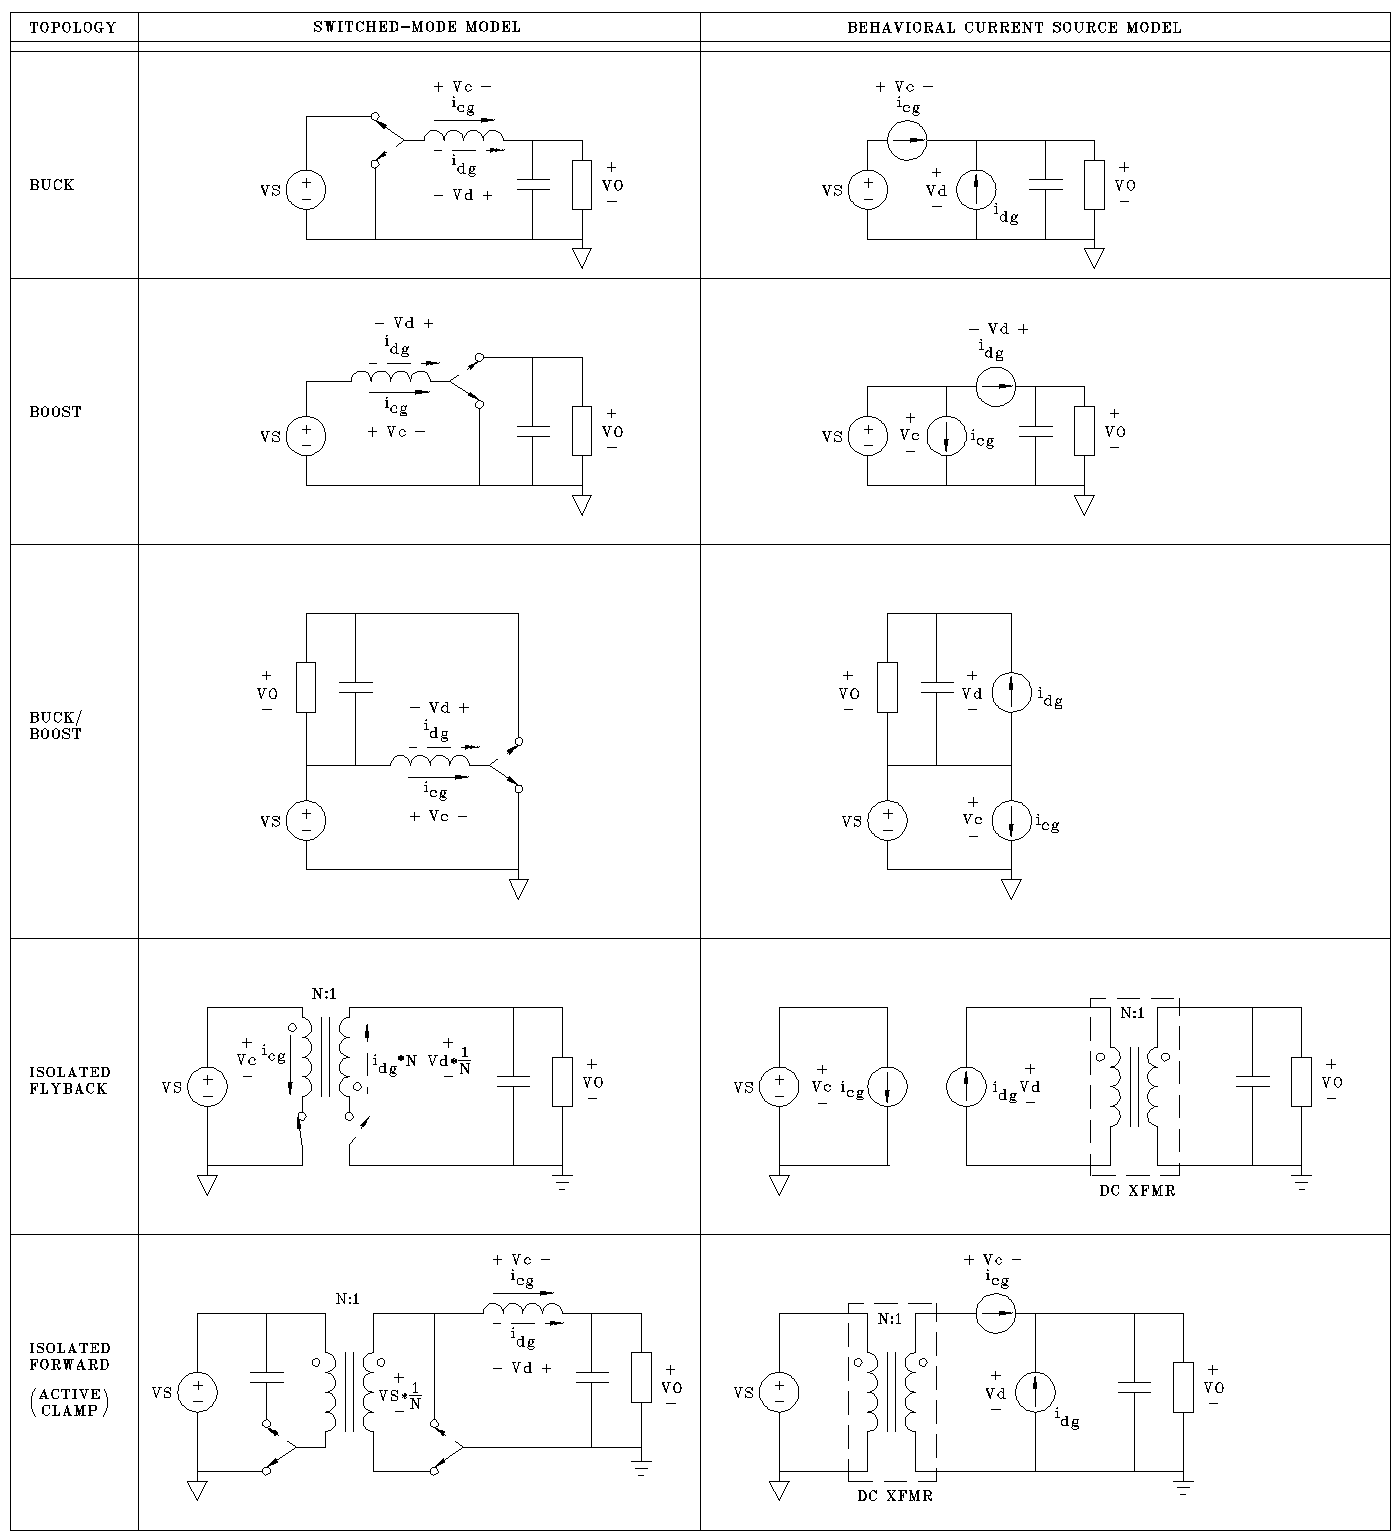
\includegraphics [
		width=16cm,
		keepaspectratio,
		] {a_SMPS_Topologies.png}}
	\caption{Review of switched-mode power converter topologies.}
	\label{fig:asmpstopologies}
\end{figure*}

\section{An Alternative Approach}
This document revisits the problem of characterizing dynamic behavior in switched mode converters. The defining feature of this approach is the use of inductor current waveform geometry to synthesize a series of cascaded filters representing the switched inductor's impulse response.  The system is synthesized as a signal processing chain involving a sampler, discrete time filters and a continuous time reconstruction filter.  Through a judicious process of sampling, re-sampling and reconstruction the inductor currents are expressed as a non-LTI filter response to the control input signal. The non-LTI filter may be evaluated directly by use of computerized numerical solvers or further developed analytically using small-signal analysis methods.

The equivalent circuit model is prepared by combining the inductor and switch together as a pair of behavioral current sources as shown in Fig. \ref{fig:asmpstopologies}. The currents $i_{cg}$ and $i_{dg}$ correspond to charging and discharging inductor currents where control-to-current transfer functions are expressed as a set of cascaded filters.  The geometry of switched current waveforms serve as a specification for the time-domain impulse responses for continuous time filters in this system's transfer function.

Several common switched inductor topologies are identified in Fig. \ref{fig:asmpstopologies} to better illustrate how this alternative model is substituted for the switch and inductor in the greater context of a switched-mode converter circuit.  

The lack of diodes shown schematically does not imply this model cannot accommodate diode behavior.  On the contrary, this switch representation generalizes the model to any type of device exhibiting switch-like behavior.  A diode, for example, is a special type of switch in which current may flow in only one direction -- the behavior defined for the current source representing the diode switch leg will account for this.  For circuits in the left-hand column of Fig. \ref{fig:asmpstopologies} one would consider the center position of the switch a legal state (no connection to either throw) so the switch could open like a diode preventing reverse current flow.

\section{Peak Current Mode Control System}
At this point the proposed approach has been prepared in a generalized form. The next step is to derive expressions for $i_c$ and $i_d$ as a function of known quantities. To this end, a specific control scheme must be considered. Rather than providing exhaustive treatment of current source behaviors for multiple control schemes, this document will focus on the peak current mode control scheme (some other texts refer to this as current programmed mode). Peak current control is chosen as an example because of the widespread availability of reference designs and switched-mode converter controller IC's using this control implementation.

Peak Current Mode Control is a technique used for controlling inductor currents in a switched-mode converter on a cycle-by-cycle decision-making interval. The control signal sets a threshold to limit inductor peak intake currents during the charging portion of the cycle. When the inductor current crosses this threshold, a latch is reset to signal shut-down of the primary switch device. A compensating ramp is often added to the inductor's current sense signal to induce pre-mature tripping of the comparator -- a tecnique used to stabilize the peak current control loop.

\begin{figure}[ht!]
	\centering
	\begin{subfigure}[t]{\columnwidth}
		\centering	
		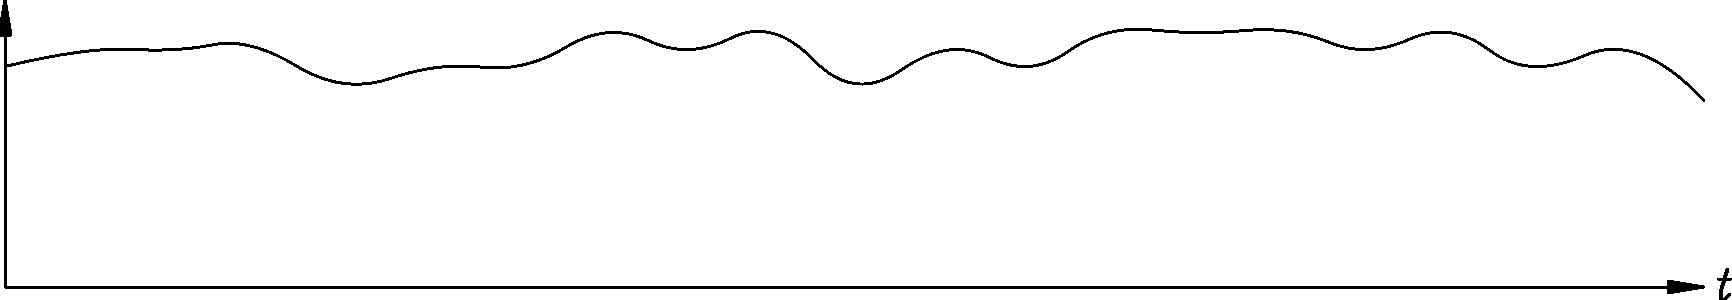
\includegraphics[
		width=\columnwidth,
		keepaspectratio,]{a_sampling_sequences/sampling_01}
		\caption{}
		\label{fig:resampling_a}
	\end{subfigure}%
	
	\begin{subfigure}[t]{\columnwidth}
		\centering	
		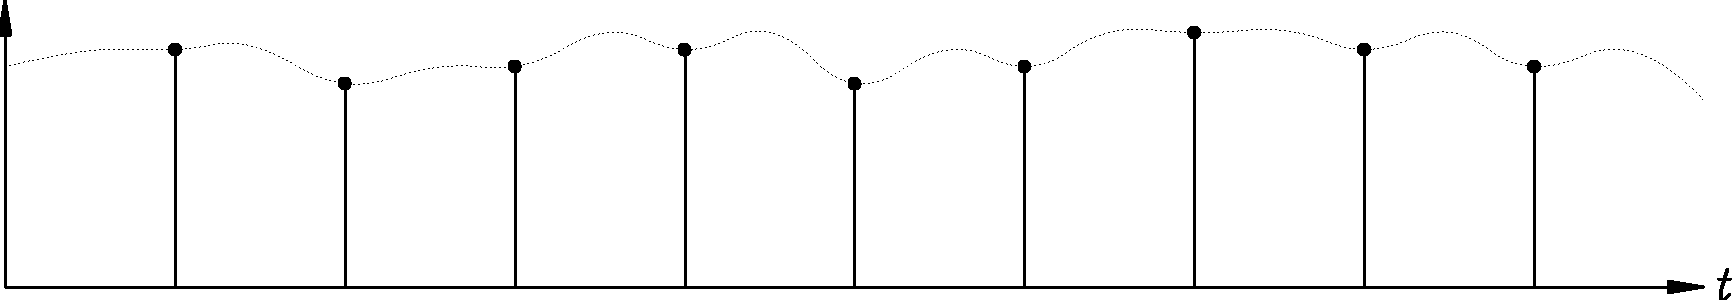
\includegraphics[
		width=\columnwidth,
		keepaspectratio,]{a_sampling_sequences/sampling_02}
		\caption{}
		\label{fig:resampling_b}
	\end{subfigure}
	
	\begin{subfigure}[t]{\columnwidth}
		\centering	
		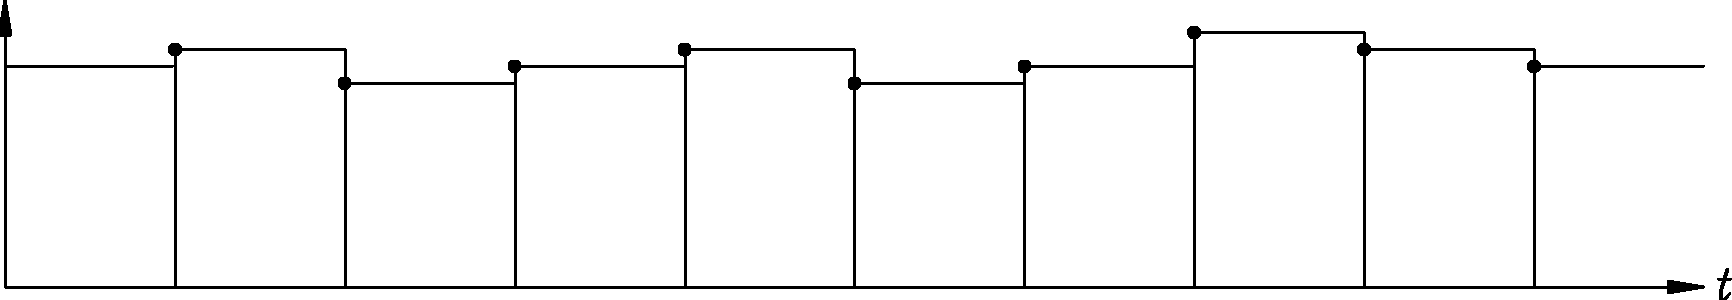
\includegraphics[
		width=\columnwidth,
		keepaspectratio,]{a_sampling_sequences/sampling_03}
		\caption{}
		\label{fig:resampling_c}
	\end{subfigure}
	
	\begin{subfigure}[t]{\columnwidth}
		\centering	
		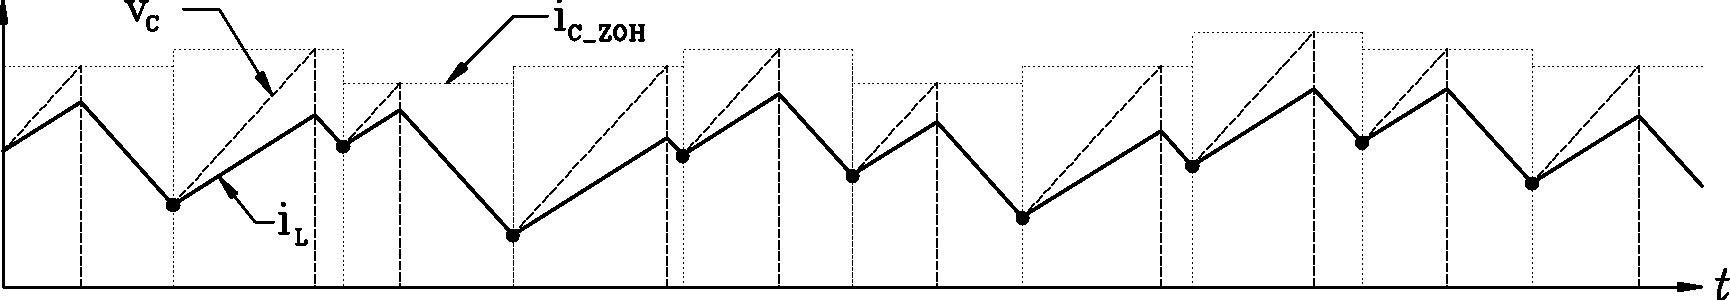
\includegraphics[
		width=\columnwidth,
		keepaspectratio,]{a_sampling_sequences/sampling_04}
		\caption{}
		\label{fig:resampling_d}
	\end{subfigure}
	
	\begin{subfigure}[t]{\columnwidth}
		\centering	
		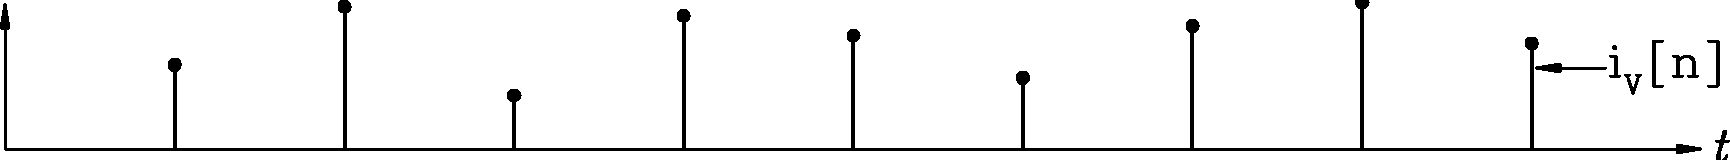
\includegraphics[
		width=\columnwidth,
		keepaspectratio,]{a_sampling_sequences/sampling_05}
		\caption{}
		\label{fig:resampling_e}
	\end{subfigure}
	
	\begin{subfigure}[t]{\columnwidth}
		\centering	
		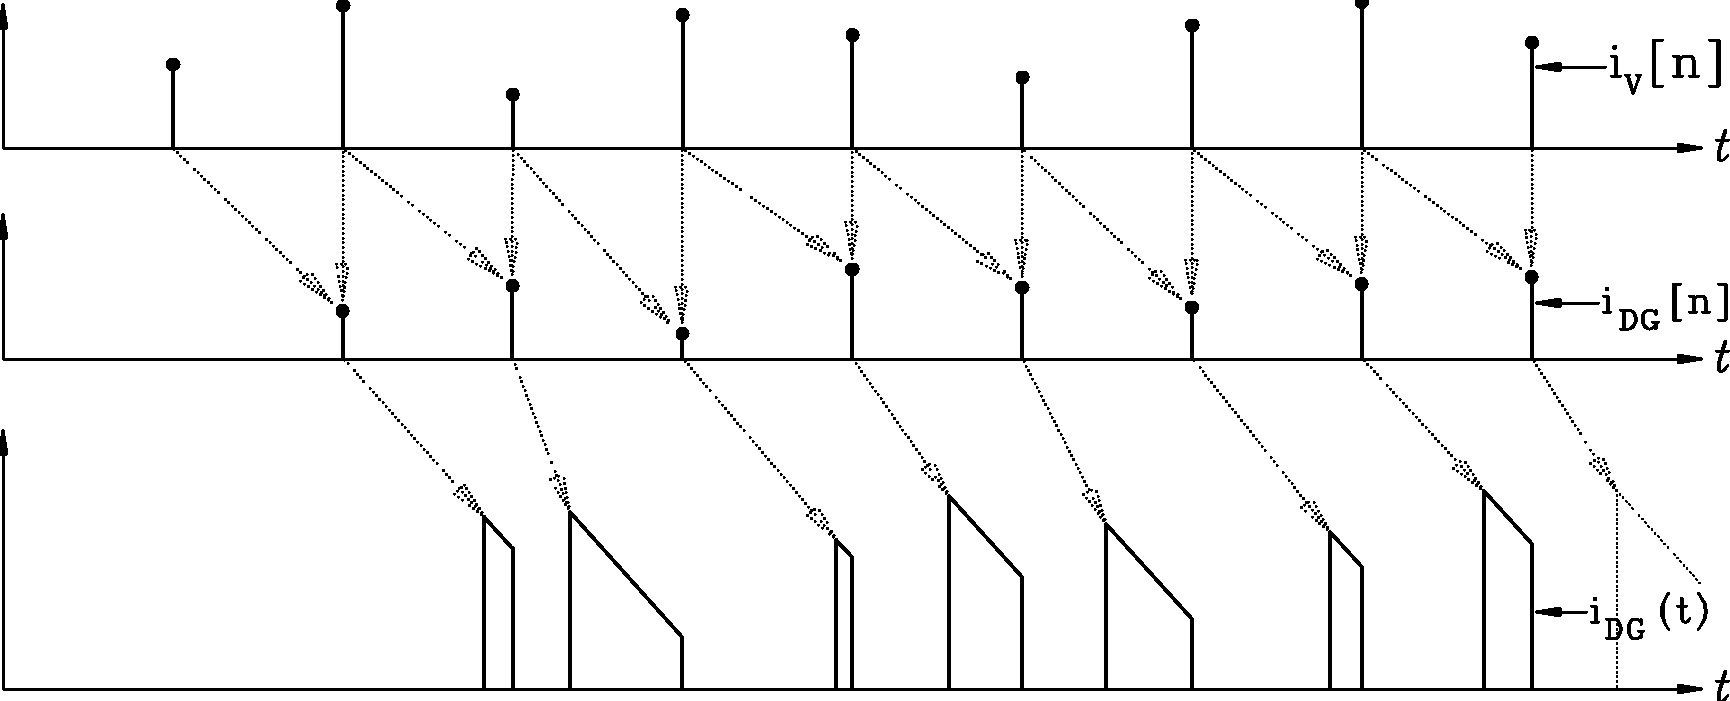
\includegraphics[
		width=\columnwidth,
		keepaspectratio,]{a_sampling_sequences/sampling_06}
		\caption{}
		\label{fig:resampling_f}
	\end{subfigure}
	
	\begin{subfigure}[t]{\columnwidth}
		\centering	
		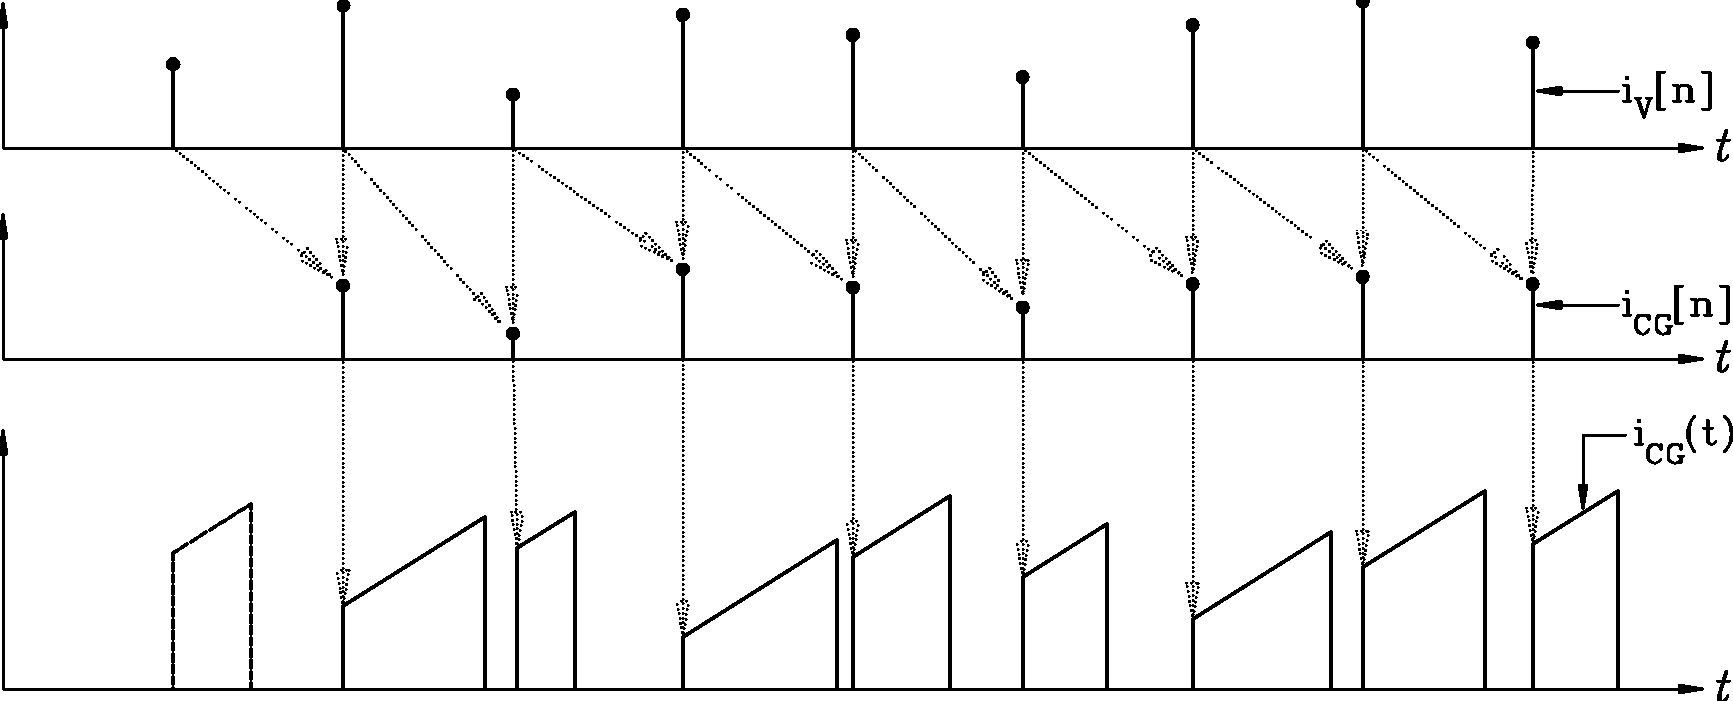
\includegraphics[
		width=\columnwidth,
		keepaspectratio,]{a_sampling_sequences/sampling_07}
		\caption{}
		\label{fig:resampling_g}
	\end{subfigure}
	
	\caption{Illustration of the analytical process used to re-sample the peak current control input (shown in (a)) and construct output currents as a system of filters with impulse responses derived from inductor current geometry. Waveform in (a) is sampled in (b), then reconstructed with Zero-Order-Hold function in (c). Inductor current is geometrically expressed in (d) and valley currents re-sampled as a discrete time signal in (e). Sequences in (f) and (g) illustrate steps used to generate system output with a set of FIR filters using valley currents as an input.}
	\label{fig:resampling}
\end{figure}

\section{Dissection of the Sampled System}
The diagram in Fig. \ref{fig:resampling} steps through the analytical process used to understand the system as a series of cascaded filters. The control input signal, $i_c(t)$ is shown in Fig. \ref{fig:resampling_a} as an arbitrary waveform with features illustrating a possibility the bandwidth of this signal may exceed the Nyquist rate.  A sampled version of this signal is illustrated in Fig. \ref{fig:resampling_b}.

The first objective is to derive a relationship between the sampled control inputs of Fig. \ref{fig:resampling_b} and valley currents shown in Fig. \ref{fig:resampling_e}. The charging currents ($i_{cg}[n]$) and discharging currents ($i_{dg}[n]$) can be expressed as an FIR filter in discrete time as shown in Fig. \ref{fig:resampling_f} and \ref{fig:resampling_g}. The discrete-time impulse train is reconstructed to a continuous time waveform by convolution with an impulse response having the same shape as the inductor currents.

The purpose for using a process involving multiple sampling, resampling and discrete time processing operations lies in considering the direct process is not a linear time-invariant operation. For example, the frequency response of an FIR filter having the shape of inductor currents is simply low-pass, rolling off at some frequency above the Nyquist rate. As is well-known from measurements made on switched-mode power supplies the open-loop transfer function has more features than what is indicated by a flat gain response up to Nyquist rate. As exaggerated by a large-signal response in Fig. \ref{fig:resampling_d}, every inductor current pulse may have a different geometry than the last, and such features are not linearly related to the peak current control signal. 

Non-LTI systems are often evaluated as LTI systems where the excitation and response are constrained to an infinitesimal perturbation centered at a steady-state operating point. This technique, known as small-signal analysis, can be applied most easily to the immediate problem in a discrete time system.  It is intuitive to evaluate discrete units of energy transferred and stored within the system per cycle. The inductor current geometry is used to relate the energy storage and release from one cycle to the next.

In the discussion of analysis steps illustrated in Fig. \ref{fig:resampling} the function illustrated in Fig. \ref{fig:resampling_c} was not fully addressed.  This step constructs a type of input signal in which the sampled value is held for the entire sampling interval. Using this assumption simplifies the geometry problem of the next step, yet the consequence is not entirely immaterial. This function is commonly known as Zero-Order-Hold (ZOH), interpreted as a moving-average FIR filter having an easily derived frequency response. The consequence of this operation is well understood and can be precisely compensated in the system transfer function.

The associative and distributive algebraic properties of convolution imply the ZOH function is canceled using a filter having a resopnse that is the reciprocal of ZOH in the frequency domain.  The strategy employed in this analysis applies the ZOH function in the time domain (Fig. \ref{fig:resampling_c}), perform a set of linear operations (Fig. \ref{fig:resampling_d}, \ref{fig:resampling_f} and \ref{fig:resampling_g}), and then apply the inverse ZOH function in the frequency domain (not illustrated) to reconstruct $i_{cg}$ and $i_{dg}$. 

\subsection{Derivation of the Discrete Time IIR Filter}
The analytical system presented in Fig.~\ref{cpm_waveforms} shows the peak current threshold being sampled synchronous to the valley currents and then held constant throughout the switching cycle.  Charging and discharging slopes are sampled values held static throughout the sampling interval, and the compensating ramp is considered linear (constant). This system is geometrically characterized using values sampled at the rising edge of the primary gate drive signal (coincident with inductor valley currents). The effect of ZOH function is reversed for all sampled values in a single operation on the valley currents using the distributive property of convolution.

\begin{figure}[ht]
	\centerline{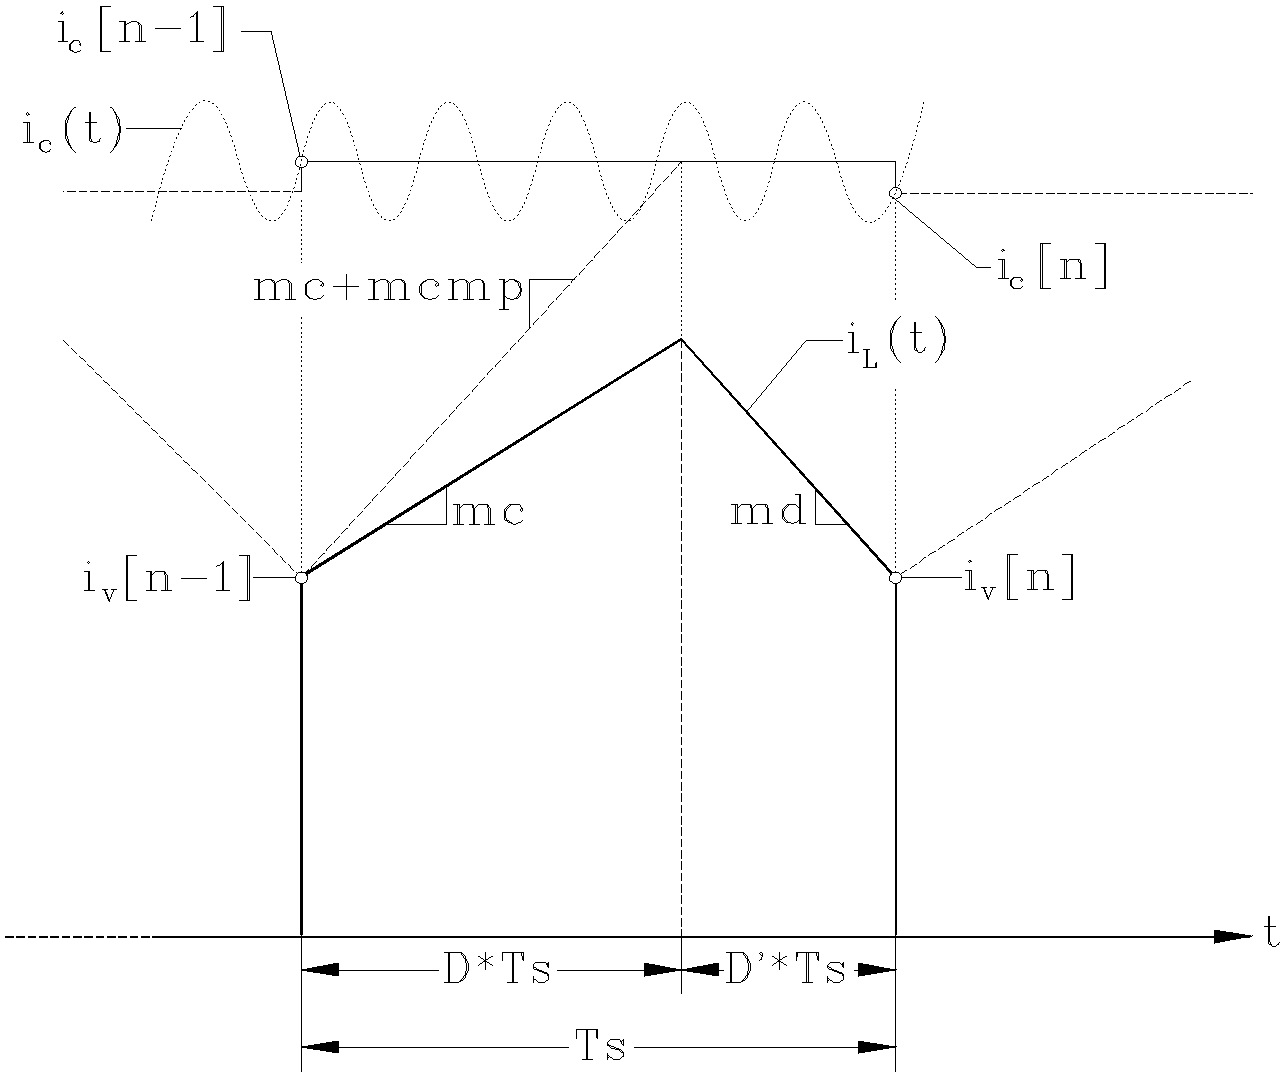
\includegraphics [
		width=7cm,
		keepaspectratio,
		] {a_cpm_waveforms.png}}
	\caption{Inductor waveforms with peak current mode control.}
	\label{cpm_waveforms}
\end{figure}

The relationship between valley currents is then,
\begin{equation}
i_v[n] =  i_v[n-1] + m_c D T_{SW} - m_d  D' T_{SW}   \label{ivd}
\end{equation} 
\begin{align*}
\text{where, } \\
T_{SW} &= \text{Modulator switching (sampling) period} \\
D &= \text{Modulator duty cycle} \\
D' &= (1-D) \\
m_c &= \text{Slope of current during charge cycle (A/s)} \\
m_d &= \text{Slope of current during discharge cycle (A/s)}\\
i_v &= \text{Inductor valley current.} \\
\end{align*}
The duty cycle can be re-expressed in the following terms,
\begin{equation}
D = \dfrac{i_c [n-1] - i_v [n-1]} {(m_c + m_{cmp})T_{SW}}
\end{equation}
\begin{align*}
\text{where, } \\
m_{cmp} &= \text{ Slope compensation (A/s)}\\
i_c &= \text{ Sampled peak current threshold.} 
\end{align*}
Then expanding $ D $ and $ D' $ in (\ref{ivd}), the following recurrence relation emerges,
\begin{equation}
i_v[n] =  \alpha i_c[n-1] + ( 1 - \alpha ) i_v [n-1] - T_{SW} m_d   \label{ivn}
\end{equation}
where,
\begin{align}
\alpha &= \frac{m_c + m_d} {m_c + m_{cmp}} \label{const_alpha}
\end{align}
It is now apparent from (\ref{ivn}) the peak current controller has the form of a discrete-time first order IIR filter. The IIR filter closely approximates the properties of a Linear Time Invariant (LTI) system under small-signal conditions in which the inductor current slopes do not change appreciably from sample-to-sample.   

\subsection{Z-transform of the Peak Current Controller}
Given a difference equation for an LTI system (as assumed in (\ref{ivn}) ) the z-transform can be evaluated by inspection.  
\begin{equation}
\mathcal{Z} \{ i_v[n] \} =  \alpha I_c(z) z^{-1} + ( 1 - \alpha ) I_v (z) z^{-1} - \mathcal{Z} \{T_{SW}m_d\}  \label{ivz}
\end{equation}

The expression in (~\ref{ivz}) is easily rearranged into a canonical form transfer function if the Z-transform of the constant term is resolved.
\begin{equation}
 \mathcal{Z} \{ T_{SW} m_d \} = 0 \label{zconst}
\end{equation}
One way to dismiss the effect of the constant seen in (\ref{ivn}) is by use of the unit step response, time shift and time reversal properties of the z-transform.

The necessary relationships are included to maintain coherence in the approach being presented.

\begin{table}[H]
	\caption{Useful Z-transform Properties}
	\begin{center}
		\begin{tabular}{|c|c|c|}
			\hline
			\textbf{Description}& \textbf{Time Domain}& \textbf{Z-tranform}\\
			\hline
			Unit Step Response & 
			u[n] =
			$ \begin{cases} 
				0 & n < 0 \\
				1 & n \geq 0 
			\end{cases} $ 
			 & U($ \mathit{z} $) = $\dfrac{1}{1-z^{-1}}$ \\
			\hline
			
			
			Time Reversal& u[-n]& U($ \mathit{z^{-1}} $) = $\dfrac{-z^{-1}}{1-z^{-1}}$  \\
			\hline
			Unit Delay & u[n-1] & $U( \mathit{z} )\mathit{z^{-1}}$ = $\dfrac{z^{-1}}{1-z^{-1}}$  \\
			\hline

		\end{tabular}
		\label{tabun}
	\end{center}
\end{table}

The choice of relationships expressed in Table \ref{tabun} plays on the following time-domain property. 
\begin{equation}
u[n-1] + u[-n] = 1 \label{funny_one}
\end{equation}
The expression in (\ref{funny_one}) is used to substitute unity in the constant expression, $ k = -T_{SW} m_d $,
\begin{equation}
	\mathcal{Z}\{ 1k \} = 
	\mathcal{Z}\{ k (u[n-1] + u[-n]) \}
\end{equation}
hence,
\begin{equation}
\mathcal{Z}\{ k \} = k \bigg( \dfrac{z^{-1}}{1-z^{-1}} + \dfrac{-z^{-1}}{1-z^{-1}} \bigg) = 0
\end{equation}

Having reasonably dismissed the constant term, (\ref{ivz}) is refactored to the following transfer function,
\begin{equation}
H_v(z) = \frac {I_v(z)} {I_c(z)} = \frac {\alpha z^{-1}} {1 - (1-\alpha) z^{-1}}  \label{hvz}
\end{equation}


\subsection{Peak Current Controller Stability Analysis}

The expression in (\ref{hvz}) becomes unstable in cases when the system is defined outside of the Region of Convergence (ROC) or the denominator approaches zero. Using Euler's formula, the complex exponential term in the denominator expands to the following.
\begin{equation}
	z^{-1} = e^{-j \omega T_{SW}} = \cos (\omega T_{SW}) - j \sin (\omega T_{SW}) 
\end{equation} 
The condition for which it is possible for the denominator to become zero is at frequency $\omega T_{SW} = \pi$, where the expression is purely real -- specifically, $e^{-j \pi} = \cos ( \pi) = -1$, so the transfer function becomes
\begin{equation}
H_V(z) \bigg|_{z=\frac{\omega_{SW}}{2}} = \dfrac{\alpha (-1)}{1 - (1 - \alpha) (-1)} = \dfrac{- \alpha}{2 - \alpha} \label{cpmstability}
\end{equation}
The condition for stability therefore requires that $\alpha < 2$.  The system is outside of the Region of Convergence (ROC) for $\alpha > 2$. It is intuitive from the time-domain expression in (\ref{ivn}) that any condition for which the magnitude of $(1 - \alpha)$ equals or exceeds 1.0, the state variable $i_v[n]$ will build rather than decay.
Recall that $\alpha$ is a function of inductor current slopes as well as the slope compensation parameter, $m_{cmp}$.  Expanding (\ref{const_alpha}) into (\ref{cpmstability}) and rearranging terms, the amount of slope compensation necessary for stability is found by ensuring the following inequality is satisfied,
\begin{equation}
m_{cmp} > \dfrac{m_d - m_c}{2} \label{slope_stab}
\end{equation}

\subsection{Comparison to Conventional Approach}
In $[ref]$ Middlebrook, Tan state the condition for stability in the peak current controller per following (with the exception that (\ref{transl_stab}) translates notation to symbols consistent with the current text.).

\begin{equation}
D'_{min} = \dfrac{0.5}{1 + \dfrac{m_{cmp}}{m_{mc}}} \label{transl_stab}
\end{equation}

For consistency with the inequality stated in (\ref{slope_stab}), the quantity in (\ref{transl_stab}) will be re-expressed as an inequality defining the values for $D'$ for which the controller is stable,
\begin{equation}
D' > \dfrac{0.5}{1 + \dfrac{m_{cmp}}{m_{mc}}} \label{transl_stab_ineq}
\end{equation}

The steady-state condition within the peak current mode controller occurs when $i_v[n] - i_v[n-1]$. Evaluation of (\ref{ivd}) in the steady state condition yields the following.
\begin{equation}
	D T_s{SW} m_c - D' T_{SW} m_d = 0 \label{dsteadystate}
\end{equation}

Substituting $D = (1-D')$, the expression in (\ref{dsteadystate}) is manipulated into the following form.
\begin{equation}
	D' = \dfrac{m_c}{m_c+m_d} \label{dp_mc_md}
\end{equation}
Combining (\ref{transl_stab_ineq}) and (\ref{dp_mc_md}),
\begin{equation}
	\dfrac{m_c}{m_c + m_d} > \dfrac{0.5}{1 + \dfrac{m_{cmp}}{m_c}} \label{tan_stab_eq}
\end{equation}
Then solving (\ref{tan_stab_eq}) for slope compensation yields the following.
\begin{equation}
	m_{cmp} > \dfrac{m_d - m_c}{2} \label{mid_stab}
\end{equation}

It is now apparent that (\ref{mid_stab}) and (\ref{slope_stab}) are in perfect agreement.

\subsection{Peak Current Controller magnitude response}
In addition to evaluating peak current controller stability the expression in (\ref{cpmstability}) may be rearranged to express a desired peak magnitude response in terms of the coefficient $\alpha$.
\begin{equation}
	\alpha =  2 \frac{|H_v(z)|}{1 + |H_v(z)|} \bigg|_{z=\frac{1}{2}\omega_{SW}} 
\end{equation}
Expanding $\alpha$ from (\ref{const_alpha}) and using additional algebraic manipulation, the amount of slope compensation corresponding to a pre-determined magnitude response is obtained.
\begin{equation}
	m_{cmp} = \frac{1 + |H_v(z)|}{2|H_v(z)|}(m_c + m_d) - m_c \bigg|_{z=\frac{1}{2}\omega_{SW}}
\end{equation}

Plotting a series of magnitude responses for values of $\alpha$ corresponding to a (notch) gain of -9 dB, increasing in 3 dB steps to +9 dB is shown below.

\begin{figure}[H]
	\centerline{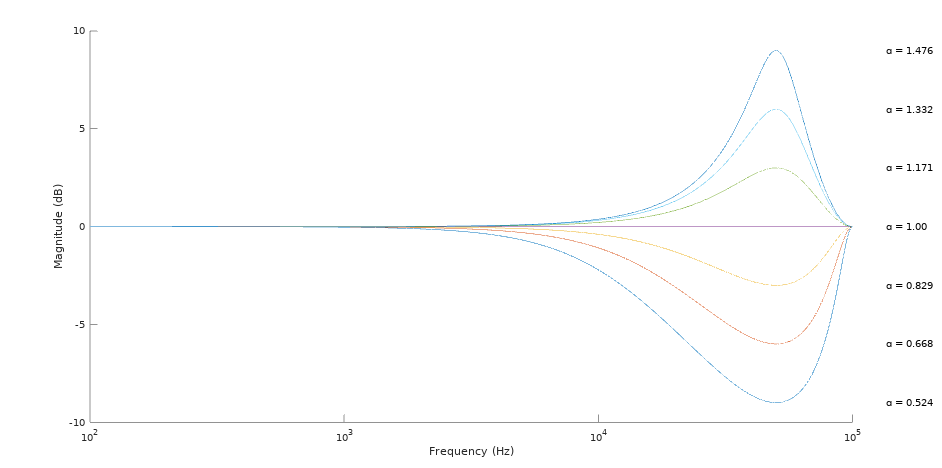
\includegraphics [
		width=9cm,
		keepaspectratio,
		] {a_Peak_Current_Controller_Response_Plot.png}}
	\caption{Peak current controller frequency response, $H_v(z)$, plots with different values of $\alpha$ ($F_{SW}=100kHz$). }
	\label{PCM_mag_resp}
\end{figure}

The utility of having slope compensation expressed as a function of peak magnitude response is apparent when considering switched-mode converter design flow.  For example, one can identify the minimum slope compensation required to achieve a desired amount of gain margin at $\frac{1}{2}F_{SW}$.

 

\begin{figure}[ht]
	\centerline{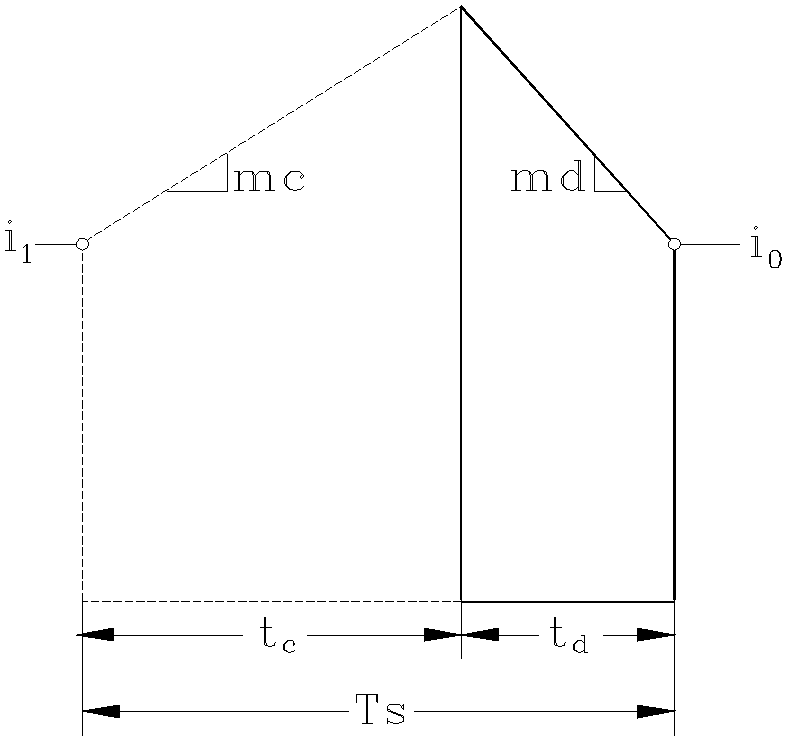
\includegraphics [
		width=5cm,
		keepaspectratio,
		] {a_discharge_current.png}}
	\caption{Inductor current waveform illustrated as a geometric problem. }
	\label{FIR_geometry}
\end{figure}

\section{Cycle Average Current as FIR Filter}
The inductor energy stored and released per switching cycle is a discrete quantity which may be expressed as a function of valley currents. If other quantities feeding into the waveform geometry are treated as sampled values (held constant over the switching interval), then the problem of relating average inductor currents to valley currents is reduced to that of a simple geometry problem as illustrated in Fig. \ref{FIR_geometry}. Since all quantities defining the inductor waveform begin and end within the same switching cycle, the valley-to-average-current transfer function response is finite and limited to a single switching cycle.

The set of parameters needed to express the area enclosed in the geometric shape illustrated in Fig. \ref{FIR_geometry}  are $i_0$, $i_1$, $m_c$, $m_d$, and $T_{SW}$. The anchor points identified as $i_0$ and $i_1$ serve as the interface linking the geometric problem to valley currents.

A noteworthy benefit of describing the discrete energy-per-cycle quantity as a function of valley current is that the system's core transfer function is agnostic to the control scheme implemented.  For example, whether voltage mode, peak-current mode, quasi-resonant or even hysteretic control, the geometric problem presented in Fig. \ref{FIR_geometry} remains unchanged.

Referring back to the equivalent circuit models presented in Fig. \ref{fig:asmpstopologies} it is apparent that the discharging and charging cycle currents must be treated as separate geometric problems if a generalized model is to be had from this approach.

\subsection{Geometric Area of Charging Current}
The average charging current is expressed as an integral of the geometric shape in Fig. \ref{FIR_geometry} over the charging interval, $t=0$ to $t=t_c$.
\begin{align}
i_{cg} = & \frac{1}{T_{SW}}\int_0^{t_c}(i_1 + m_c t)dt \label{icg_integral}
\end{align}
The integral expressed in (\ref{icg_integral}) evaluates to the following:
\begin{align}
i_{cg} = & \frac{t_c}{T_{SW}} i_1 + \frac{m_ct_c^2}{2T_{SW}} \label{icg_eval}
\end{align}
It is necessary to further expand (\ref{icg_eval}) in terms of defined system constants and signals.  To this end, the following equality is easily derived by inspection of Fig. \ref{FIR_geometry}.

\begin{equation}
m_ct_c+i_1 = m_d(T_{SW} - t_c)+i_0\\ \label{tc_equality}
\end{equation}

Where (\ref{tc_equality}) is used to solve for the unknown, $t_c$, in terms of known quantities.

\begin{equation}
t_c = \frac{i_0-i_1+T_{SW}m_d}{m_c+m_d} \label{tcharge}
\end{equation}	

Substituting (\ref{tcharge}) into (\ref{icg_eval}) the following solution for \(i_{cg}\) is obtained with sufficient use of algebraic simplification.
\begin{equation}
i_{cg} = a_{cg}i_0^2+b_{cg}i_1^2+c_{cg}i_0i_1+d_{cg}i_0+e_{cg}i_1+f_{cg} \label{i_cg_canon}
\end{equation}
Where the constants are expanded per below,
\begin{align*}
a_{cg} = & \frac{1}{2T_{SW}} \bigg[ \frac{m_c}{m_c^2+2m_cm_d+m_d^2} \bigg]\nonumber\\
b_{cg} = & -\frac{1}{2T_{SW}} \bigg[ \frac{m_c + 2m_d}{m_c^2+2m_cm_d+m_d^2} \bigg]\nonumber\\
c_{cg} = & \frac{1}{T_{SW}} \bigg[  \frac{m_d}{m_c^2+2m_cm_d+m_d^2} \bigg] \nonumber\\
d_{cg} = & \frac{m_cm_d}{m_c^2+2m_cm_d+m_d^2}\nonumber\\
e_{cg} = & \frac{m_d^2}{m_c^2+2m_cm_d+m_d^2}\nonumber\\
f_{cg} = & \frac{T_{SW}}{2} \bigg[ \frac{m_c m_d^2}{m_c^2+2m_cm_d+m_d^2} \bigg]\nonumber\\
\end{align*}

\subsection{Geometric Area of Discharging Current}
The process for finding a canonical solution for the discharging current follows the same process used for finding the average charging current. In this case the problem is simplified by reversing the shape in Fig. \ref{FIR_geometry} and evaluating an integral having the same form as (\ref{icg_integral}), substituting $i_0$, $m_d$ and $t_d$ for the initial current, slope and time variable.
\begin{align}
i_{cg} = & \frac{1}{T_{SW}}\int_0^{t_d}(i_0 + m_d t)dt \label{idg_integral}
\end{align}
The integral in (\ref{idg_integral}) evaluates to the following.
\begin{align}
i_{dg} = & \frac{t_d}{T_{SW}} i_0 + \frac{m_dt_d^2}{2T_{SW}}
\label{idg_integral_eval}
\end{align}

Using the identity $t_d = T_{SW} - t_c$, (\ref{idg_integral_eval}) becomes the following.
\begin{align}
i_{dg} = & \frac{ T_{SW} - t_c}{T_{SW}} i_0 + \frac{m_d( T_{SW} - t_c)^2}{2T_{SW}}
\label{idg_noncanon}
\end{align}
and then substituting (\ref{tcharge}) into (\ref{idg_noncanon}), the solution for \(i_{dg}\) is seen to have the same form as (\ref{i_cg_canon}), differing only by the set of coefficients characterizing the familiar polynomial expression.
\begin{equation}
i_{dg} = a_{dg}i_0^2+b_{dg}i_1^2+c_{dg}i_0i_1+d_{dg}i_0+e_{dg}i_1+f_{dg} \label{i_dg_canon}
\end{equation}
Where the constants are expanded per below.
\begin{align*}
a_{dg} = & - \bigg (\frac{1}{2T_{SW}} \bigg)  \frac{2m_c + m_d}{m_c^2+2m_cm_d+m_d^2}  \nonumber\\
b_{dg} = &  \bigg ( \frac{1}{2T_{SW}} \bigg ) \frac{m_d}{m_c^2+2m_cm_d+m_d^2}  \nonumber\\
c_{dg} = & \bigg ( \frac{1}{T_{SW}} \bigg ) \frac{m_c}{m_c^2+2m_cm_d+m_d^2} \nonumber\\
d_{dg} = & \frac{m_c^2}{m_c^2+2m_cm_d+m_d^2}\nonumber\\
e_{dg} = & \frac{m_c m_d}{m_c^2+2m_cm_d+m_d^2}\nonumber\\
f_{dg} = & \bigg ( \frac{T_{SW}}{2} \bigg ) \frac{m_c^2 m_d}{m_c^2+2m_cm_d+m_d^2}
\end{align*}

\subsection{Small-Signal Analysis of the Non-LTI Inductor Currents}
It is no surprise (\ref{i_cg_canon}) and (\ref{i_dg_canon}) follow the same form since the geometric shapes are fundamentally similar. This commonality affords the convenience of having a generalized solution for the small signal model since the charging and discharging currents differ only in specific values used for the coefficients.

The formulae expressed in (\ref{i_cg_canon}) and (\ref{i_dg_canon}) constitute a pair of non-LTI FIR filters when the geometric shape represents inductor current, specifically,
\begin{align}
i_0 &= i_v[n] \nonumber \\
i_1 &= i_v[n-1]
\label{i0i1ivn}
\end{align}

This system can be understood as an LTI filter if the signals and response are constrained to infinitesimal amplitude, as though operating on a linear tangent at a point on the quadratic curve. This treatment of nonlinear systems is more commonly known as small-signal analysis, and treated in greater detail in [ref].

In this document discussion of small-signal analysis theory will be omitted, but the mechanics of this technique are introduced as a segue into the analysis.  Considering the general form of a nonlinear function, $y = f(x)$, the function is approximated as linear at an operating point $x_0$.  The approximation becomes increasingly accurate as deviations from $x_0$ are reduced in amplitude.

The linearized function is expressed using a partial derivative of $f(x)$ with respect to $x$,
\begin{equation}
	G_{lin} = \frac{\partial f(x)}{\partial x}\bigg|_{x=x_0}
\end{equation}
Where $G_{lin}$ is the equivalent linear gain on small deviations about $x_0$. In this case, $x$ can be reinterpreted as,
\begin{equation}
y \approx f(x_0) + \Delta_x G_{lin}
\end{equation}
where $\Delta_x$ represents a small perturbation superimposed on $x$ when biased at operating point $x_0$.  Since DC offsets within the transfer function are already captured in steady-state analysis, the small-signal transfer function is simplified to express only changes about the operating point, more specifically,
 \begin{equation}
 \Delta_y = \Delta_x G_{lin} \label{ss_transfer}
 \end{equation}
where $\Delta_y$ is the amount of change in $y$ due to a small change in $x$ with DC offsets absent from the expression; therefore, (\ref{ss_transfer}) is the small-signal transfer function for $y=f(x)$.

Now having briefly outlined the process, this will be applied to the generalized form of (\ref{i_cg_canon}) and (\ref{i_dg_canon}). Below the quantity $i_{avg}$ is used as a placeholder for $i_{cg}$ and $i_{dg}$ to generalize the expression.

\begin{equation}
i_{avg} = a i_0^2+b i_1^2+c i_0i_1+d i_0+e i_1+f  \label{i_av_gen}
\end{equation}

In this case there are two independent variables, $i_0$ and $i_1$, so the partial derivative must be evaluated for both variables. One helpful observation is when considering the system is operating in a small-signal steady-state the preceding IIR filter stage is also presumed operating in this state, hence $i_v[n] = i_v[n-1] = i_{v\infty}$, where $i_{v\infty}$ is used to identify the final steady-state value for the valley current.

\begin{align}
\Delta{_{avg}} &= \Delta{_0}\frac{\partial i_{avg}}{\partial i_0}\bigg|_{i_1=i_{v\infty}} + \Delta{_1}\frac{\partial i_{avg}}{\partial i_1}\bigg|_{i_0=i_{v\infty}} 
  \label{i_av_deriv}
\end{align}

where,
\begin{align}
	\Delta_0 & \text{ represents a small change in } i_0 \nonumber \\
	\Delta_1 & \text{ represents a small change in } i_1 
	\label{deltai0i1}
\end{align}
and the partial derivatives represent the small-signal gain on each input parameter.

Now let us consider the cycle-averaged output current to be the following,
\begin{equation}	
	i_{avg} \approx I_{\infty} + \Delta_{avg}
\end{equation}

where $I_{\infty}$ is the steady-state average current obtained given the condition that control input, $i_c[n]$, is held constant and $i_v[n]$ is allowed to settle to its final steady state operating point as expressed in the following.

\begin{equation}
	i_{v\infty} = \lim_{n \to \infty} i_{v}[n] = \lim_{n \to \infty}  i_{v}[n-1]
	\label{ivinf}
\end{equation}

Then $i_{avg}$ from (\ref{i_av_gen}) is evaluated using (\ref{i0i1ivn}) and (\ref{ivinf}),
\begin{equation}
	I_{\infty} = i_{avg} \bigg|_{\stackrel{i0=i_{v \infty}}{i1=i_{v \infty}}} = a i_{v \infty}^2+b i_{v \infty}^2+c i_{v \infty}i_{v \infty}+d i_{v \infty}+e i_{v \infty}+f 
\end{equation}

which simplifies to the following after collecting like terms,

\begin{equation}
I_{\infty} = (a + b +c)i_{v \infty}^2 + (d+e)i_{v \infty} + f
\label{iavg_steady_state}
\end{equation}

Now having the DC gain of the FIR filter, the gain on small perturbations about this operating point remains to be determined.  For this,  (\ref{i_av_gen}) is evaluated using terms defined in (\ref{deltai0i1}) as substituted into (\ref{i_av_deriv}).

\begin{align}
	\Delta_{avg} &= 
	\frac{\partial}{\partial i_0} 
	\bigg [
	a i_0^2+b i_1^2+c i_0i_1+d i_0+e i_1+f \bigg ] 
	\Delta_0 \bigg |_{i_0=i_{v\infty}} \nonumber \\
	&+ 
	\frac{\partial}{\partial i_1} 
	\bigg [
	a i_0^2+b i_1^2+c i_0i_1+d i_0+e i_1+f \bigg ] 
	\Delta_1 \bigg |_{i_1=i_{v\infty}}
	\label{avgdelta_partial}
\end{align}
Evaluating (\ref{avgdelta_partial}) results in the following expression for small-signal changes in average currents.

\begin{equation}
	\Delta_{avg} = \big ( 2 a i_{v\infty} + c i_{v\infty} + d  \big) \Delta_0 + 
	\big ( 2 b i_{v\infty} + c i_{v\infty} + e  \big) \Delta_1
	\label{adelta_LTI}
\end{equation}
In which the parenthetical expressions from (\ref{adelta_LTI}) represent a set of coefficients which are further abstracted per the following.
\begin{align}
k_0 = 2 a i_{v\infty} + c i_{v\infty} + d \nonumber \\
k_1 = 2 b i_{v\infty} + c i_{v\infty} + e 
\end{align}
Recall geometrically the quantity $\Delta_{avg}$ is a small change to the area bounded by the inductor current waveform during a single switching cycle as a function of small changes to the anchor points $i_0$ and $i_1$, expressed as $\Delta_0$ and $\Delta_1$. The geometry problem has been set up for re-interpretation using a symbolic convention consistent with more widely known literature.

\begin{equation}
		\hat{i}_{avg} = k_0 \hat{i}_v[n] + 
	k_1 \hat{i}_v[n-1]
	\label{avg_FIR}
\end{equation}
Where the circumflex notation (e.g. $\hat{i}[n]$) represents the AC small-signal response of a nonlinear system. The proposed translation is executed by interpreting the $\Delta_{avg}$, $\Delta_0$, and $\Delta_1$ as peak-to-peak limits on arbitrary AC waveforms $\hat{i}_{avg}$, $\hat{i}[n]$ and $\hat{i}[n-1]$, respectively. Interpreting the geometric problem as shown in (\ref{avg_FIR}) has a more easily identifiable form of a first-order FIR filter.

The form of the FIR filter expressed in (\ref{avg_FIR}) is expanded to an expression of the AC transfer function between valley currents and average output currents for both charging and discharging cycles by substituting coefficients identified in (\ref{i_cg_canon}) and (\ref{i_dg_canon}), specifically,
\begin{equation}
\hat{i}_{cg} = k_{0_{cg}} \hat{i}_{v}[n] + 
k_{1_{cg}} \hat{i}_v[n-1]
\label{avg_FIR_cg}
\end{equation}
for the charging cycle current, and
\begin{equation}
\hat{i}_{dg} = k_{0_{dg}} \hat{i}_{v}[n] + 
k_{1_{dg}} \hat{i}_v[n-1]
\label{avg_FIR_dg}
\end{equation}
represents the discharging cycle current.

\subsection{Continuous Time Approximation of FIR Averaging Filter}
A well-documented phenomenon of the switched inductor discharge current response (commonly associated with a flyback topology) is the right-half-plane-zero (RHPZ) that shows up in the loop response.  The system evaluated according to the equivalent circuit models of Fig. \ref{fig:asmpstopologies} indicates the RHPZ exists in buck and forward converters but its response is swamped by the complementary left-half-plane zero characteristic of the charging cycle current.

To give intuitive context for the following derivation the FIR responses of (\ref{avg_FIR_cg}) and (\ref{avg_FIR_dg}) are plotted as discrete-time systems overlaid with the corrected response (inverse ZOH), and continuous time approximation (conventional RHPZ).

\subsubsection{Derivation of the conventional RHPZ}
From above plots it is apparent the impulse response based approach presented in this document traces the shape of the RHPZ as presented in conventional literature [ref]. It is here shown how the well-known RHPZ expression is readily obtained by evaluating (\ref{avg_FIR_dg}) in the limit as $T_{SW} \to 0$.

First an intermediate variable is defined,
\begin{equation}
g_{dg} = \frac{1}{m_c^2+2m_cm_d+m_d^2}
\end{equation} 

which is a quantity common in every coefficient found in the discharging current polynomial expressed in (\ref{i_dg_canon}). Now the small-signal FIR filter in (\ref{avg_FIR_dg}) can be neatly expanded as follows.

\begin{equation}
\hat{i}_{dg}[n] = (2a+c)i_{v\infty} \hat{i}_{v}[n] + d + 
(2b+c)i_{v\infty} \hat{i}_v[n-1] + e
\label{avg_FIR_dg_expanded}
\end{equation}

Then substituting $a$, $b$, $c$, $d$ and $e$ from coefficients of (\ref{i_dg_canon}),

 \begin{align}
 \frac{\hat{i}_{dg}[n]}{g_{dg}} = &-\frac{m_c + m_d}{T_{SW}} i_{v\infty} \hat{i}_{v}[n] + m_c^2 \hat{i}_v[n-1] \nonumber \\ 
 &+ \frac{m_c + m_d}{T_{SW}} \hat{i}_v[n-1] + m_c m_d \hat{i}_v[n-1]
 \label{avg_FIR_dg_expanded_coeffs}
 \end{align}
 
Re-expressing the difference equation in the continuous time domain with further rearrangement exposes a form of the derivative definition,

\begin{align}
	\frac{\hat{i}_{dg}(t)}{g_{dg}} =&  -\frac{\hat{i}_v(t) - \hat{i}_v (t-T_{SW})} {T_{SW}}
	(m_c + m_d) i_{v\infty} \nonumber \\
	&+	( m_c^2 + m_c m_d ) \hat{i}_v(t-T_{SW}) 
	\label{idg_t_differential_def}
\end{align}

The expression in (\ref{idg_t_differential_def}) exposes a differential equation if considering what happens when sampling frequency approaches infinity.
	
\begin{equation}
\lim_{T_{SW} \to 0} \frac{\hat{i}_{dg}(t)}{g_{dg}} = -(m_c + m_d) i_{v\infty} \frac{d \hat{i}_v(t)}{dt}
+ 	( m_c^2 + m_c m_d ) \hat{i}_v(t) 
\end{equation}

The Laplace transform is then obtained by inspection,

\begin{equation}
	 \frac{\hat{I}_{dg}(s)}{g_{dg}} =  - (m_c + m_d) i_{v\infty}\hat{I}_{v}(s)s + ( m_c^2 + m_c m_d ) \hat{I}_{v}(s)
\end{equation}

Finally a transfer function is defined,

\begin{equation}
H_{dg} (s) = \frac{\hat{I}_{dg}(s)}{\hat{I}_{v}(s)} =  g_{dg} (m_c + m_d) 
\big (\frac{m_c}{i_{v\infty}} - s \big )
\label{RHPZ_s_raw}
\end{equation}

The conventional notion of a continuous time RHPZ is now apparent in (\ref{RHPZ_s_raw}).  
Further algebraic manipulation is required to see it in its well-known form.  The first item to re-express is the steady-state valley current, $i_{v\infty}$, which must be re-expressed in terms of the steady-state $i_{dg}$ if $R_{out} = V_{dg}/i_{dg}$ is to be pulled out of this expression.

\begin{equation}
	i_{dg} = \frac{L_m}{2V_{dg}T_{SW}} (i_{pk}^2 - i_{v\infty}^2)
	\label{steady_state_idg}
\end{equation}

where $i_{pk}$ is the peak current, so the following substitution may be used.

\begin{equation}
i_{pk} = i_{v\infty} + \Delta_R
\label{ipk_ripple}
\end{equation}

The quantity $\Delta_R$ is the steady-state ripple observed during CCM operation, further expanded to the following expression.

\begin{equation}
\Delta_R = \frac{V_{cg}V_{dg}}{V_{cg} + V_{dg}} \frac{T_{SW}}{L_m} =
D'\frac{V_{dg} T_{SW}}{L_m}
\label{steady_state_ripple}
\end{equation}

Substituting (\ref{steady_state_ripple}) and (\ref{ipk_ripple}) into (\ref{steady_state_idg}), the following is obtained.

\begin{align}
i_{dg} =& \frac{L_m}{2V_{dg}T_{SW}} \bigg(2\Delta_R i_{v\infty} + \Delta_R^2 \bigg) \nonumber \\
=& \frac{L_m}{2V_{dg}T_{SW}} \bigg(2 D'\frac{V_{dg} T_{SW}}{L_m} i_{v\infty} + \bigg(D'\frac{V_{dg} T_{SW}}{L_m}\bigg)^2\bigg) \nonumber \\
=&  D' i_{v\infty} + D'^2\frac{V_{dg} T_{SW}}{L_m}
\end{align}

Recall this system has been evaluated in the limit as $T_{SW} \to 0$, so the steady-state relationship between $i_{dg}$ and $i_{v\infty}$ simplifies to the following.

\begin{align}
i_{dg} = D' i_{v\infty}
\end{align}

Now, from (\ref{RHPZ_s_raw}) the location of the right-half-plane zero is extracted per following.

\begin{equation}
	\omega_{RHPZ} = \frac{m_c}{i_{v\infty}} = \frac{V_{cg}}{L_m} \frac{D'}{i_{dg}}
	\label{wrhpz_raw}
\end{equation}

A little more work is needed to obtain the canonical continuous-time expression for the RHPZ location, specifically, re-casting $V_{cg}$ in terms of $V_{dg}$.

\begin{equation}
V_{cg} = V_{dg} (\frac{1}{D} - 1)
\label{vcgdg_equivalence}
\end{equation}

Then substituting (\ref{vcgdg_equivalence}) into (\ref{wrhpz_raw}) the following emerges.

\begin{align}
	\omega_{RHPZ} =& \frac{V_{dg}}{ i_{dg} L_m } D' (\frac{1}{D} - 1) \nonumber \\
	=& \frac{R_{OUT}}{L_m} (\frac{D'}{D} - D') \nonumber \\
	=&  \frac{R_{OUT}}{L_m D} D'(1-D) \nonumber \\
	=& \frac{D'^2}{L_m D} R_{OUT}
	\label{WHRPZ_canonical}
\end{align}

It is now apparent the expression in (\ref{WHRPZ_canonical}) exactly matches the expression given in [ref].


\subsection{Impulse Response Analysis}
The IIR filters characterized by (\ref{avg_FIR_cg}) and (\ref{avg_FIR_dg}) are a discrete time representation of charging and discharging currents, resampled as averaged values.  Information missing from the discrete time system includes high-frequency response and group delay (phase) associated with the real output current pulse shape. However, the small signal change from cycle-to-cycle has now been captured by the discrete-time transfer functions relating peak-control, valley and average currents. The final step in reconstructing the complete impulse response is performed by convolving the discrete time system output pulse train with a continuous-time FIR filter, having impulse response shape identical to that of the inductor current geometry.  The steady-state inductor current pulse shape includes information about the high-frequency response as well as the filter group delay.  The steady-state inductor current pulse may be considered analogous to a digital-to-analog converter's reconstruction filter. 

\subsubsection{Frequency Response of Discharging Current}

\subsubsection{Frequency Response of Charging Current}

\section{Conclusion}

Example inline citation
\cite{b1}, is a citation.


\begin{thebibliography}{00}
\bibitem{b1} Reference 1.
\bibitem{b2} Reference 2.
\end{thebibliography}


\end{document}
